\section{Confounding in LLM Evaluation}
\label{sec:confounding}

\begin{figure}[t]
\centering
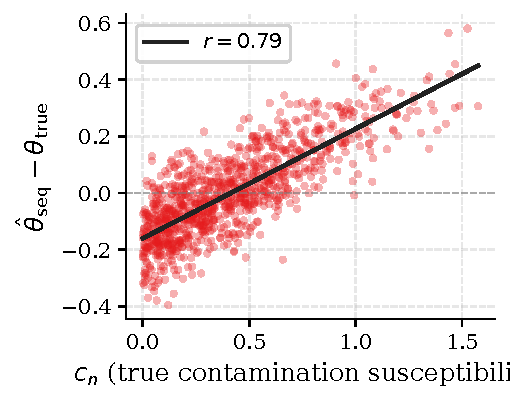
\includegraphics[width=\columnwidth]{fig2_ovb_bias}
\caption{Sequential estimation bias ($\hat{\theta}_{\mathrm{seq}} - \theta_{\mathrm{true}}$) versus true contamination susceptibility $c_n$. Pearson $r = 0.79$ ($p < 0.001$) confirms systematic overestimation of contaminated models. Synthetic data: $N = 50$, $I = 100$, $J = 8$.}
\label{fig:ovb_bias}
\end{figure}

The Many-Facet Rasch Model (MFRM) extends classical Rasch measurement to settings with multiple rater facets \citep{linacre1989mfrm, linacre1994mfrm}. Originating in educational measurement, the model treats rater variation as a nuisance facet to be estimated and removed rather than a source of noise to be averaged over. In the LLM evaluation context, where $J$ judges score $N$ models across $I$ items, the MFRM specifies
%
\begin{equation}
\label{eq:mfrm}
\log \frac{P(Y_{nij} \geq k \mid \theta_n, b_i, d_j, \gamma_k)}{P(Y_{nij} < k \mid \theta_n, b_i, d_j, \gamma_k)} = \theta_n - b_i - d_j - \gamma_k,
\end{equation}
%
where $Y_{nij}$ is the ordinal rating by judge $j$ for model $n$ on item $i$, $\theta_n$ is the ability of model $n$ ($n = 1, \ldots, N$), $b_i$ is the difficulty of item $i$ ($i = 1, \ldots, I$), $d_j$ is the severity of judge $j$ ($j = 1, \ldots, J$), and $\gamma_k$ is the threshold for category $k$. All facets reside on a common logit scale, so model ability is directly comparable after adjustment for item difficulty and judge severity. \citet{jiao2025mfrm_llm} applied this framework to compare ten LLM raters with human experts and showed that MFRM separates genuine ability from systematic judge effects in multi-judge panels.

However, standard MFRM assumes that all systematic sources of score variation are captured by the modeled facets. This assumption breaks down when some models have been exposed to benchmark items during training \citep{dcr2025}. Such contamination inflates scores on exposed items through memorization rather than genuine ability. We represent this effect as an interaction $c_n \cdot e_i$, where $c_n \geq 0$ is the contamination susceptibility of model $n$ and $e_i \in [0, 1]$ is the exposure level of item $i$. The complete data-generating process becomes
%
\begin{equation}
\label{eq:full}
\eta_{nijk} = \theta_n - b_i - d_j - \gamma_k + c_n \cdot e_i.
\end{equation}


When a practitioner fits the standard MFRM (Eq.~\ref{eq:mfrm}) to data generated by Eq.~\ref{eq:full}, the contamination term is absent from the estimated model. Its influence does not vanish but is absorbed into the estimated parameters $\tilde{\theta}_n$, $\tilde{b}_i$, and $\tilde{d}_j$, which distorts all downstream inferences.

The consequence of this omission can be stated precisely.

\begin{observation}[Omitted Variable Bias in MFRM]
\label{obs:ovb}
Let the full model be $\eta_{nijk} = \theta_n - b_i - d_j - \gamma_k + c_n \cdot e_i$ and the short model omit the contamination term: $\tilde{\eta}_{nijk} = \tilde{\theta}_n - \tilde{b}_i - \tilde{d}_j - \gamma_k$. Under a linear approximation to the ordinal logit link \citep{wooldridge2010, angrist2009mostly},\footnote{The OVB formula is exact for linear models. We apply it to the MFRM linear predictor $\eta$, which is an approximation. Synthetic validation confirms the approximation quality: the Pearson correlation between the predicted bias direction and empirical bias reaches $r = 0.79$ ($p < 0.001$); the linear result accurately characterizes bias direction and relative magnitude.}
\begin{equation}
\label{eq:ovb}
\mathrm{plim}(\tilde{\theta}_n - \theta_n) = \delta_n \cdot c_n,
\end{equation}
where $\delta_n$ depends on the projection of the exposure vector $(e_i)$ onto the design matrix of the short model (explicit form in Appendix~\ref{app:gamma}). The bias is non-zero whenever $\mathrm{Cov}(d_j,\, c_n \cdot e_i) \neq 0$. This captures the confounding component; in the nonlinear MFRM, a specification bias from omitting $c_n \cdot e_i$ persists even at zero covariance (Section~\ref{sec:experiments}).
\end{observation}

While the OVB framework provides the analytical lens for understanding \emph{why} omitting contamination biases ability estimates, our empirical results (Section~\ref{sec:experiments}) reveal that the bias magnitude is driven primarily by the specification error itself rather than the exposure-severity covariance term---a finding that strengthens the case for joint modeling regardless of the covariance structure. G-MFRM uses the full nonlinear likelihood; the linear approximation serves only as directional motivation. Monte Carlo simulation confirms that bias magnitude is approximately constant across confounding levels $\rho$ (Figure~\ref{fig:bias_vs_rho}): omission of $c_n \cdot e_i$, not its correlation with $d_j$, is the primary driver. Joint estimation reduces the bias slope by ${\sim}$69\% at all $\rho$ levels. Neither sequential ordering resolves this: bias-first approaches \citep{cyclicjudge2026} absorb contamination into $\hat{\theta}$, while contamination-first approaches \citep{dcr2025} misattribute judge severity as contamination ($r = 0.79$, $p < 0.001$; Figure~\ref{fig:ovb_bias}).

\begin{figure}[t]
\centering
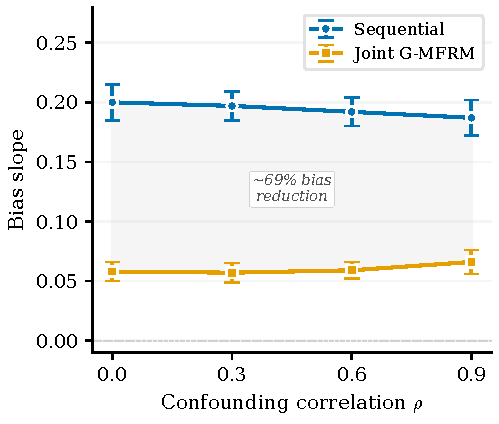
\includegraphics[width=\columnwidth]{fig4_bias_vs_rho}
\caption{Sequential estimation bias is approximately constant across confounding levels $\rho$, confirming that omission of the contamination term, not its correlation with judge severity, drives the bias. Joint G-MFRM reduces the bias slope by ${\sim}$69\% at all $\rho$ levels. Synthetic data: $N = 50$, $I = 100$, $J = 8$.}
\label{fig:bias_vs_rho}
\end{figure}